In this section we consider the ranked tie-breaking rule, 
and present a series of single threshold strategies with their guarantees. 
We then show an interesting connection to the setting of a single agent that can choose up to $k$ rewards. 
We start by presenting the single threshold strategies.
 
\begin{theorem}\label{thm:prophet_serial_threshold_inequality}
	For every $i\leq n$ and $\ell=0, \ldots, n-i$, let $\hat{T}_i^\ell=\frac{1}{\ell+2}\sum_{j=i}^{i+\ell} \E [y_j]$. 
	The single threshold strategy $\hat{T}_i^\ell$ (i.e., select $v_t$ iff $v_t\geq \hat{T}_i^\ell$) guarantees an expected utility of at least $\hat{T}_i^\ell$ for the $i$-ranked agent.	
%For agent $i$, the threshold strategy $\hat{T}_i^\ell=\frac{1}{\ell+2}\sum_{j=i}^{i+\ell} \E [y_j]$ for $0 \leq \ell\leq n-i$  gives a $\hat{T}_i^\ell$-guarantee. 
\end{theorem}
\begin{proof}
	Fix an agent $i$. Let $S_{-i}$ be the strategies of all agents except agent $i$, and let $S=(\hat{T}_i^\ell,S_{-i})$.
	Let $\assignn{i}{j}{S}$ denote the event that agent $i$ is assigned the reward $v_j$ in strategy profile $S$. I.e., $\assignn{i}{j}{S}$ is the event that agent $i$ competed over reward $v_j$ and received it according to the ranked tie-breaking rule. 
	For simplicity of presentation, we omit $S$ and write $\assign{i}{j}$.
	We bound the utility of agent $i$ under strategy profile $S$.
	\begin{eqnarray*}
	  u_i(S)  & = & \E\left[ \sum_{j=1}^{n}{v_j\cdot\Pr\left(\assign{i}{j}\right)}\right]    \nonumber \\ 
	 & =& \E\left[\sum_{j=1}^{n}{(\hat{T}_i^\ell+v_j-\hat{T}_i^\ell)\Pr\left(v_j\geq \hat{T}_i^\ell,\forall_{r<j} \overline{\assign{i}{r}},\assign{i}{j}\right)}\right]. \nonumber 
	\end{eqnarray*}

Let $p=\sum_{j=1}^{n} \Pr(v_j\geq \hat{T}_i^\ell,\forall_{r<j}  \overline{\assign{i}{r}},\assign{i}{j})$ (i.e., $p$ is the probability that agent $i$ receives some reward in strategy profile $S=(\hat{T}_i^\ell,S_{-i})$), and let $Z^{+}=\max\{Z,0\}$.
We can now write $u_i(S)$ as follows:
\begin{eqnarray}
	 u_i(S)	  & = & p \cdot\hat{T}_i^\ell + \E\left[\sum_{j=1}^{n}{(v_j-\hat{T}_i^\ell)^+\Pr\left(\forall_{r<j} \overline{\assign{i}{r}},\assign{i}{j}\right)}\right] \nonumber \\
	& \geq & p \cdot  \hat{T}_i^\ell \label{eq:1} + \E\Bigl[\sum_{j=1}^{n}(v_j-\hat{T}_i^\ell)^+ \Bigr.  
	 \left. \cdot (1-p)\cdot\Pr\left(\assign{i}{j} \mid \forall_{r<j}\overline{\assign{i}{r}}\right)\right] \nonumber\\
%\end{eqnarray}
%\begin{eqnarray}
	& \geq & p\cdot \hat{T}_i^\ell + (1-p)\cdot \E\left[\sum_{j=i}^{n}(y_j-\hat{T}_i^\ell)^+\right] \label{eq:2}\\
	& \geq & p\cdot \hat{T}_i^\ell + (1-p)\cdot \E\left[\sum_{j=i}^{i+\ell}(y_j-\hat{T}_i^\ell)\right] \nonumber\\
	& = & p\cdot \hat{T}_i^\ell + (1-p)\cdot \left( \E\left[\sum_{j=i}^{i+\ell}y_j\right]-(\ell+1)\hat{T}_i^\ell \right)\nonumber\\
	& = & p\cdot \hat{T}_i^\ell + (1-p)\cdot \left((\ell+2)\cdot \hat{T}_i^\ell-(\ell+1)\cdot\hat{T}_i^\ell \right) = \hat{T}_i^\ell. \nonumber
	%& = & p\cdot \E\left[\sum_{j=i}^{i+\ell} \frac{y_j}{\ell+2}\right] + (1-p)\cdot\E\left[\sum_{j=i}^{i+\ell} \frac{y_j}{\ell+2}\right] = \hat{T}_i^\ell,
	\end{eqnarray}
	
	%The first inequality holds since the probability of not getting any reward until time $j$ is bounded by $1-p$ (i.e., the probability of not getting any reward). 
	%The last inequality holds since if $v_j-T^\ell\geq 0$ and agent $i$ is still active, the reward is selected, thus assigned with probability at least $1/k$. 
	
	Inequality \eqref{eq:1} holds since the probability of not getting any reward until time $j$ is bounded by $1-p$ (i.e., the probability of not getting any reward). 
	Inequality \eqref{eq:2} holds since there are at most $i-1$ agents that are ranked higher than agent $i$, therefore there are at most $i-1$ rewards that can be selected but not assigned to agent $i$.
	Finally, the last equality holds by the definition of $\hat{T}_i^\ell$.		
\end{proof}

The special case of Theorem~\ref{thm:prophet_serial_threshold_inequality} where $\ell=0$ gives the following corollary.
\begin{corollary}
For every $i$, the threshold strategy $\hat{T}_i^0$ guarantees an expected utility of $\frac{\E[y_i]}{2}$ for the $i$-ranked agent.
\end{corollary}

We next show that the bound in Theorem~\ref{thm:prophet_serial_threshold_inequality} is tight.
\begin{proposition}\label{pro:lb_serial}
	For every $\epsilon>0$ and every $i \leq n$, there exists an instance such that in the unique equilibrium of the game, the $i$-ranked agent gets an expected utility of at most $\frac{1}{\ell+2}\sum_{j=i}^{i+\ell} \E [y_j]+\epsilon$ for every $\ell \leq n-i$.
\end{proposition}

\begin{proof}
	Given some $\epsilon>0$ and $i \leq n$, consider the following instance (depicted in Figure~\ref{fig:ranked}): 
	$$
	v_t = 
	\begin{cases}
	\infty & \text{ for } t < i\\
	1 & \text{ for } i \leq t < n \\
	\frac{1+\epsilon}{\epsilon} \mbox{ w.p. } \epsilon, \mbox{ and } 0  \mbox{ w.p. } 1-\epsilon& \text{ for } t = n
	\end{cases}
	$$
	One can easily verify that in the unique equilibrium of the game, agents $1, \ldots, i-1$ will be assigned rewards $v_1,\ldots,v_{i-1}$, and agent $i$ will be assigned the last reward $v_n$ for an expected utility of $1+\epsilon$.
	It holds that:
	$$ u_i(S) = 1+\epsilon = \frac{\E[\sum_{j=i}^{i+\ell}y_j]}{2+\ell}+\epsilon.$$
\end{proof}

\begin{figure}[h!]
	\centering
	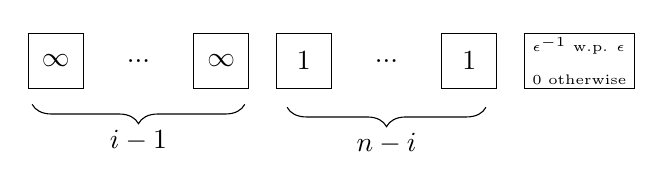
\begin{tikzpicture}[scale=0.35]
	\draw (0,0) rectangle node (G) {$\infty$} ++(2,2); 
	\draw [draw=white](3,0) rectangle node (dots) {...} ++(2,2); 
	\draw (6,0) rectangle node (J) {$\infty$} ++(2,2); 
	\draw (9,0) rectangle node (C) {$1$} ++(2,2); 
	\draw [draw=white](12,0) rectangle node (dots) {...} ++(2,2); 
	\draw (15,0) rectangle node (A) {$1$} ++(2,2); 
	\draw (18,0) rectangle node (B)[align=left] {\tiny${\epsilon}^{-1}$ w.p. $\epsilon$\\\tiny$0$ otherwise} ++(4,2); 
	\draw[decorate,decoration={brace, amplitude=7pt, raise=10pt, mirror}]
	(C.south west) to node[black,below= 16pt] {$n-i$} (A.south east);%
	\draw[decorate,decoration={brace, amplitude=7pt, raise=10pt, mirror}]
	(G.south west) to node[black,below= 16pt] {$i-1$} (J.south east);%
	\end{tikzpicture}
	\caption{An example where the expected reward for agent $i$ is no more than $\frac{1}{\ell+2}\sum_{j=i}^{i+\ell} \E [y_j]+\epsilon$}
	\label{fig:ranked}
\end{figure}

%\TBD{check if the say it or refer to it (\citet{KleinbergW19} HajiaghayiKS07 kennedy1987prophet?)}
We next show that for any instance, the set of rewards assigned to the $k$ competing agents in equilibrium coincides with the set of rewards that are chosen by the optimal algorithm for a single decision maker who can choose up to $k$ rewards and wishes to maximize their sum. 
\citet{KleinbergW19} show that the only optimal strategy of such a decision maker, takes the form of $nk$ dynamic thresholds, $\{T_t^i\}_{i,t}$ for all $t\leq n$ and $i \leq k$, so that the agent accepts reward $v_t$ if $v_t \geq T_t^i$, where $k-i$ is the number of rewards already chosen (i.e., $i$ is the number of rewards left to choose)\footnote{The uniqueness holds for distributions with no mass points. For distributions with mass points, whenever $v_t=T_t^i$, the decision maker is indifferent between selecting and passing.}. Moreover, they show that these thresholds are monotone with respect to $i$.

%Recall that this is the only optimal strategy up to cases where $v_t=T_t^i$.
%\begin{observation}[\citet{KleinbergW19}]
%	For every $t \leq n$ and $i \leq k$, $T_t^i\geq T_t^{i+1}$.
%\end{observation}

With the characterization of the strategy of a single decision maker who can choose up to $k$ rewards, we can characterize the unique SPE for the $k$-agent game\footnote{The SPE is unique up to cases where $T_j^i=v_t$; in these cases the agent is indifferent.}.
\begin{theorem}\label{thm:propht many lex is like a single agent}
Let $\{T_t^i\}_{i \in [k],t \in [n]}$ be the optimal strategy of a single decision maker who may choose up to $k$ rewards and wishes to maximize their sum. The unique SPE of the $k$-agent game is for agent $i$ to accept $v_t$ iff $v_t \geq T_t^{i'+1}$, where $i'\leq i$ is the rank of agent $i$ among the active agents. This SPE is unique up to cases where $v_t = T_t^{i'}$.
\end{theorem}
\begin{proof}
	Let $S^i$ denote the optimal strategy of the single agent who may choose up to $i$ rewards, as described above. 
	Let $S_i$ be the strategy of agent $i$ as described in the assertion of the theorem.
	We prove by induction that for every $i \in [k]$, the rewards that are chosen by agents $1,\ldots,i$ correspond to the rewards chosen by a single decision maker, who may choose up to $i$ rewards, and uses strategy $S^i$. 
	For the case of $i=1$, the claim holds trivially. %, since the settings are the same.
	Assume the claim holds for any number of agents smaller than $i$. 
	Since agent $i$ has no influence on the rewards received by agents $1,\ldots,i-1$, we may assume that agents $1,\ldots,i-1$ are playing according to strategies $S_1,\ldots,S_{i-1}$.
	
	%Let $S^i$ be the optimal strategy for a single decision maker who may choose up to $i$ awards.
	For every $i\in [k]$, the total utility of agents $1,\ldots,i$ is bounded by the utility of the single decision maker $u(S^i)$, since the single decision maker can simulate a game with $i$ competing agents. Hence, by the induction hypothesis, agent $i$ can obtain a utility of at most $u(S^i)-u(S^{i-1})$. By playing according to $S_i$, we are guaranteed that whenever at least $j$ agents are still active, any reward $v_t$ such that $v_t \geq T_t^{j}$ will be taken by one of the agents. Thus, when every agent $i$ is playing according to $S_i$, players $1, \ldots, i$ play according to $S^i$. Consequently, their total utility is $u(S^i)$, and the utility of agent $i$ is then maximal. The uniqueness (up to the cases where $v_j = T_j^{i'}$) is by the uniqueness of the optimal strategy of the single decision maker.     
\end{proof}

We note that by Theorem~\ref{thm:prophet_serial_threshold_inequality} it holds that
in the unique SPE described in Theorem~\ref{thm:propht many lex is like a single agent}, every agent  $i$ receives at least $\max_{\ell=0}^{n-i} \frac{1}{\ell+2}\sum_{j=i}^{i+\ell} \E [y_j]$. 

Using the results of \citet{alaei2011bayesian} regarding a single decision maker choosing $k$ rewards, we deduce an approximation of the social welfare in equilibrium:
%By the algorithm of \citet{alaei2014bayesian} we can deduce an approximation of the social welfare:
\begin{corollary} \label{cor:welfare_prophet}
	In SPE of the $k$ agent prophet game, the expected social welfare is at least $1-O(\frac{1}{\sqrt{k}})$ of the optimal welfare.
\end{corollary}

